%%%%%%%%%%%%%%%%%%%%%%%%%%%%%%%%%%%%%%%%%%%%%%%%%%%%%%%%%%%%%%%%%%%%%%
% Sovereign AI
% Author: Prof. Dr.-Ing. Mark Schutera
% Based on Tufte-style layout
\makeindex
%%%%%%%%%%%%%%%%%%%%%%%%%%%%%%%%%%%%%%%%%%%%%%%%%%%%%%%%%%%%%%%%%%%%%%

% A hands-on buildbook. The running example is one real rig: a platform
% designed for four GPUs, populated today with a single RTX 3090, expandable
% by dropping cards in. Tone borrows the reflective framing of Philosophy of
% AI but the body is weighted toward Missing Semester hands-on: bill of
% materials, verbatim commands, config files, a verifiable artifact per block.
%
% Series spine (chapters 02-06 are currently commented out below):
%   01 The Rig               hardware, design for four, one 3090, wired and unpowered
%   02 The Engine            first boot, Ubuntu Server, driver, Docker, Ollama, Open WebUI
%   03 Everywhere            Tailscale / Cloudflare exposure + Open WebUI API keys
%   04 A Voice in the House  Home Assistant + Wyoming + Whisper + Piper + Ollama
%   05 Second Brain          Obsidian on the local engine
%   06 Next Steps            multimodal, OCR, retrieval, images, and beyond
% See outline.md for the chapter plans.

\documentclass{../sharedAssets/tufte}

%%
% Book metadata
% Long title on the title page, short form in the running header and metadata.
% Title and subtitle are one \title argument, split by an explicit \\: the class
% sets the whole thing letterspaced allcaps at 36pt, so the subtitle carries its
% own \fontsize to drop it back to a readable second line. No space after \\ (it
% would survive as an indent in the letterspaced line).
\title[Sovereign AI]{Owning the Mind\\{\fontsize{16}{20}\selectfont Your guide to sovereign AI at home}}
\author[\defaultauthor]{\defaultauthor}
\publisher[\defaultpublisher]{\defaultpublisher}
\renewcommand{\notesdir}{notes_sovereignai}

% Load optional fonts
\loadoptionalfonts

% Build photos live in figures/; the class only puts graphics/ on the path.
\graphicspath{{graphics/}{figures/}{figures/cutouts/}{figures/cutouts_gray/}{figures/cutouts_hl/}}

% Schusterjungen and Hurenkinder. LaTeX defaults both penalties to 150, which is
% advisory, so single lines do get stranded at a page break. 10000 forbids them.
% \brokenpenalty stops a page breaking right after a hyphenated line.
\clubpenalty=10000
\widowpenalty=10000
\displaywidowpenalty=10000
\brokenpenalty=10000

% Additional packages
% Keeps a heading from being stranded with a line or two at a page foot, which
% also drags that section's marginnotes into the bottom margin.
\usepackage{needspace}
\usepackage{pifont}
\usepackage{amsmath}
\usepackage{soul}
\usepackage{textcase}
\usepackage{enumitem}
\usepackage{tabularx}
\usepackage{tikz}
\usetikzlibrary{positioning,fit,shapes.geometric,shapes.symbols,arrows.meta,calc,backgrounds}
\usepackage{pgfplots}
\pgfplotsset{compat=1.18}
\usepackage{float}
\usepackage{algorithm}
\usepackage{algpseudocode}
\usepackage{qrcode}
% Break long URLs anywhere so href'd citation links in the narrow Tufte
% margins wrap instead of running off the side of the page.
\usepackage{xurl}
\Urlmuskip=0mu plus 1mu\relax

\begin{document}

\makestandardfrontmatter
% Dedication
\makededication{\openepigraph{``There ain't no such thing as a free
lunch.''}{The Moon Is a Harsh Mistress, Robert A. Heinlein}}
\tableofcontents

% Introduction
\makeintroduction{%
  \newthought{Compute moved off your desk.}\index{cloud} For most of computing history a program ran
  on hardware you owned. First the data moved into the cloud. Now the models run there
  too, on a meter, and what you send is retained unless you have contracted otherwise. Both things that you should own, 
  your data and your compute, are now liabilities, and you have to pay for the privilege
  while relying on someone else's good faith.

  \newthought{Sovereignty is not autarky.}\index{sovereignty}\index{sovereign AI} National AI plans\index{national AI plans} do not propose building
  the whole stack on their home turf. They name dependencies and the levers held against
  them\cite{bakkerEurope2031}. Europe holds the lithography that prints the world's
  chips, the United States most of the compute and the leading, frontier model weights. 
  Most European plans though fund domestic compute to keep a lever of their own\cite{bakkerDeltaplan2025}.

  \newthought{A household is the same shape.} You depend on the grid, a line, a fab in
  Taiwan, and weights someone else trained. What changes is which decisions are yours once you own the infrastructure the model runs on. This book is about building a household-scale private AI stack, from the metal up, which changes the dependencies to:
  \begin{itemize}[topsep=0.25em, itemsep=0.15em, parsep=0em]
    \item cost paid once, then metered in kilowatt hours, not tokens;
    \item inference and data residency\index{data residency} on machines you own;
    \item acquired technical knowledge and skills;
    \item weights\index{model weights} on your own disk, and owning of the design space of your pipeline.
  \end{itemize}

  \marginnote{\newthought{This build is for inference.}\index{inference}\index{training}
  AI inference loads model weights once and then streams tokens, so a single
  PCIe~3.0 lane keeps up. Training, fine tuning\index{fine-tuning} and image or video
  generation\index{image generation} move tensors across the bus for the whole run. 
  When facing the latter use-case you should target a server platform auch as an AMD EPYC\index{AMD EPYC} board, which gives
  six cards a full x16 link each.}

  \newthought{Your own machine is the lever you can build today.} 
  All you need are some parts, this manual, and some tinkering. 
  From then on the model runs where you put it, on data that stays where you put
  it. You pick the model, the quantisation\index{quantization}, the runtime, and the moment to change any
  of them.
  }

%% Start the main matter
\mainmatter
\authorinrectoheader

% ----------------------------------------------------------------------
% SOVEREIGN AI, a household-scale private AI stack, built from the metal up
% ----------------------------------------------------------------------

% CHAPTER 1: the rig, hardware, design for four, one 3090, wired and unpowered
% !TEX root = ../notes_sovereignai.tex
% Chapter 1: The Rig, a build manual.
% One microsection per part, in assembly order: name the part, say what its
% datasheet numbers buy the rig, then fit it. Rationale, alternatives, and
% background live in marginnotes. Every part cites its datasheet. No prices in the
% part sections: the only figure is the day one total in the chapter opening, so
% the chapter cannot go stale line by line.
%
% The parts that are populated onto the board while it lies flat, the processor
% and cooler, the memory, and the drives, are SUBSECTIONS of The Motherboard,
% because that is one bench job in the assembly order rather than four. Its "fit
% it" paragraph, "Work on it flat", is the lead in to them. Parts that attach to
% the finished board or hang off the frame stay top level sections.
%
% Scope stops at the wired machine. Firmware setup and the enumeration probe are
% the first thing software does to the rig, so they live in the Engine chapter,
% which owns everything from the first power-on onward. Nothing here switches
% the machine on.
%
% The main column builds a ONE CARD machine, start to finish. Everything about
% growing to four cards lives in the closing "Cards Two to Four" section, which is
% the potential next extension, not part of today's build. Do not let expansion
% mechanics back into the part sections.
%
% Two closing sections follow the build, both alternative paths rather than work
% the reader does today: "Cards Two to Four" scales the rig up, "The Minimal Viable
% Rig" scales it down to a Raspberry Pi for a reader who wants every step of this
% book without the silicon. The Pi section keeps the same three newthought shape
% and the same scope rule: it stops at the assembled, unpowered board.
%%%%%%%%%%%%%%%%%%%%%%%%%%%%%%%%%%%%%%%%%%%%%%%%%%%%%%%%%%%%%%%%%%%%%%

\index{rig}\index{GPU}\index{graphics card|see{GPU}}\index{RTX 3090}\index{PCIe}%
\index{power supply}\index{sovereign AI}\index{VRAM}\index{video memory|see{VRAM}}
\chapter{The Rig}
\printchapterversion{01_hardware}
\newthought{Owning the Metal.}
\vspace{1.5em}

\newthought{This chapter builds one machine}: An open frame rig with a single
RTX~3090 and its 24~GB, which is enough to serve a capable model for private usage.
The rest of the setup is designed in a way so it is able to grow with your needs.
Order the parts in Table~\ref{tab:bom}\index{bill of materials} and fit them in the order of the sections
that follow, until the last cable is seated and the machine is ready to be switched
on. Day one is roughly 2500~euro and a few hours plugging.

\newthought{The parts list} is the Ryzen configuration of a proven quad~3090 local
AI home server, priced at 3000~EUR when it was built by me in 2026.

% Full width table*: the tabular spans the text block AND the margin column, but the
% caption still sets in the margin, below the table. Nothing else may occupy the
% margin at that height: a marginnote or a citation footnote landing there prints
% straight through the caption with no LaTeX warning. That is why the cited
% paragraph sits ABOVE the table, so its footnote clears the caption.
% Column widths are fractions of \linewidth, which is the full measure in here.
\vspace{2\baselineskip}
\begin{table*}[!ht]
\centering
\begin{tabular}{p{0.24\linewidth}p{0.58\linewidth}p{0.10\linewidth}}
    \toprule
    \textbf{Component} & \textbf{Part} & \textbf{Pieces} \\
    \midrule
    Frame & open GPU rack frame & 1 \\
    Motherboard & Gigabyte B650 Eagle AX & 1 \\
    CPU & AMD Ryzen 5 9600X, AM5 & 1 \\
    CPU cooler & AM5 tower air cooler & 1 \\
    Memory & G.SKILL Ripjaws S5 64\,GB DDR5-6000 & 1 \\
    Storage & NVMe Gen4 x4 2\,TB, M.2 2280 & 1 \\
    GPU & RTX~3090 24\,GB, used & 1 (4) \\
    Risers, x1 & PCIe 3.0 x1 riser, cards 2 to 4 & 0 (3) \\
    Power supply & ASRock PG-1600G, 1600\,W & 1 \\
    \bottomrule
\end{tabular}
\vspace{1.5em}
\caption{The bill of materials, in the order the parts go together. A bracketed
number is what this board, frame, and supply will carry later.} \label{tab:bom}
\end{table*}

% ==============================================================================================
% THE MOTHERBOARD
% ==============================================================================================

\newpage
\section{The Motherboard}\index{motherboard}\index{mainboard|see{motherboard}}\index{PCIe!lanes}

\newthought{A Gigabyte B650 Eagle AX}\index{Gigabyte B650 Eagle AX}, a mainstream board that support our design
decisions \cite{gigabyteB650EagleAX}:

\marginnote{\newthought{A slow slot} therefore costs seconds per model swap, while
this does not touch inference, we still care.}

\begin{itemize}[topsep=0.25em, itemsep=0.4em, parsep=0em]
    \item To support the processor we will be choosing, the socket must be AM5\index{AM5 socket}.
    \item For the GPU the top x16 slot\index{PCIe!x16 slot} is best when running the sixteen PCIe lanes,
    short for peripheral component interconnect express, straight from the processor
    rather than through the chipset\index{chipset}. A model's whole weight file crosses that link
    every time it loads, so model swapping\index{model swapping} will benefit from this wiring.
    \item Four slots have to be x16 sized, so we can grow the server in terms of GPU
    later on. Total VRAM\index{VRAM}, the video memory on the cards themselves, is the ceiling
    on model size, and we can extend that by up to 4 GPUs with this characteristics.
    \item For storage we need one M.2 socket\index{M.2 socket} wired PCIe~4.0~x4 or better straight
    from the processor, and this board has three, so a second drive later costs
    nothing today. That one drive carries everything the server accumulates, model
    weights, container volumes, embeddings, documents, and everything else data.
\end{itemize}

\begin{figure}[!ht]
\centering
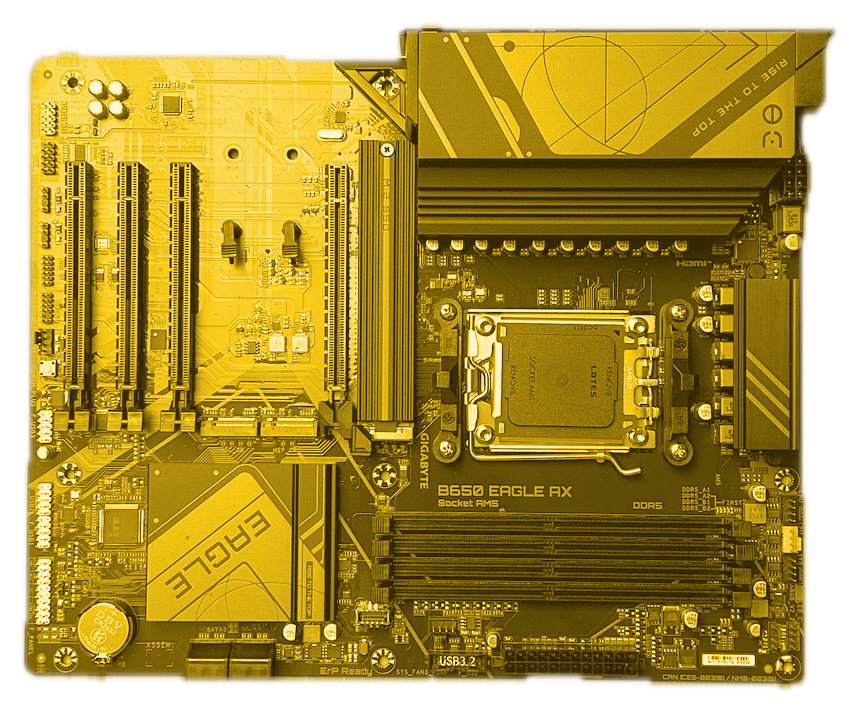
\includegraphics[width=0.45\linewidth]{01_board_bare_flat_hl}
\caption{Gigabyte B650 Eagle AX}\label{fig:board}
\end{figure}

\newthought{Work on it flat.} Lay the board on its own box, on the antistatic bag\index{antistatic bag} it
shipped in, and populate it there: Processor, cooler, memory, and the drive all go
in. This manual guides you step by step.

\marginnote{\newthought{Read the manuals.} Every part ships one, and it holds the
pin maps, socket order, and slot wiring that no build guide reproduces correctly.}

% ==============================================================================================
% THE PROCESSOR AND COOLER
% ==============================================================================================

\vspace{1.5em}
\needspace{9\baselineskip}
\subsection{The Processor and Cooler}

\newthought{An AMD Ryzen 5 9600X}\index{Ryzen 5 9600X}\index{CPU}, paired with an AM5 tower air cooler\index{air cooler}, a modest chip
that supports our design decisions\cite{amdRyzen9600X}.

\marginnote{\newthought{Why a tower and not a low profile block.} An open frame has
no lid, so the height a tower needs costs nothing here, and there is no case airflow
for a flat block to borrow either. And towers are also more efficient 
and quieter than flat blocks.}

\begin{itemize}[topsep=0.25em, itemsep=0.4em, parsep=0em]
    \item For inference we need very little compute on the CPU. Six Zen~5\index{Zen 5} cores, twelve threads, 3.9~GHz base and up to 5.4 boost, 32~MB
    of L3, and a 65~watt default thermal design power\index{thermal design power}, is perfect for this.  The GPUs carry the real work while the processor only feeds them and runs the container
    workloads layered on top.
    \item For the top slot to run a real x16, PCIe has to come from the processor
    itself rather than through the chipset.
    \item For the display we want integrated graphics\index{integrated graphics} on the chip itself, so the
    monitor never has to occupy a slot, and a 3090 stays free for the inference and AI model load.
    \item For the cooler we need an AM5 tower air cooler. The fan on the front of the fin stack sits over
    the first memory slot, so a fan with adjustable positioning is smart.
\end{itemize}

\begin{figure}[!ht]
\centering
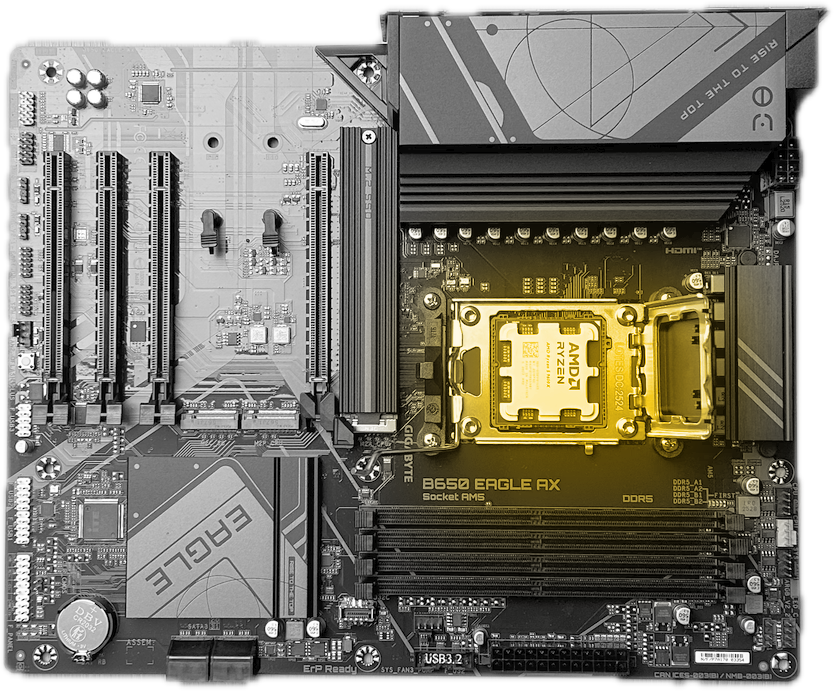
\includegraphics[width=0.45\linewidth]{02_board_cpu_seated_hl}
\caption{AMD Ryzen 5 9600X, AM5}\label{fig:cpu}
\end{figure}

\begin{figure}[!ht]
\centering
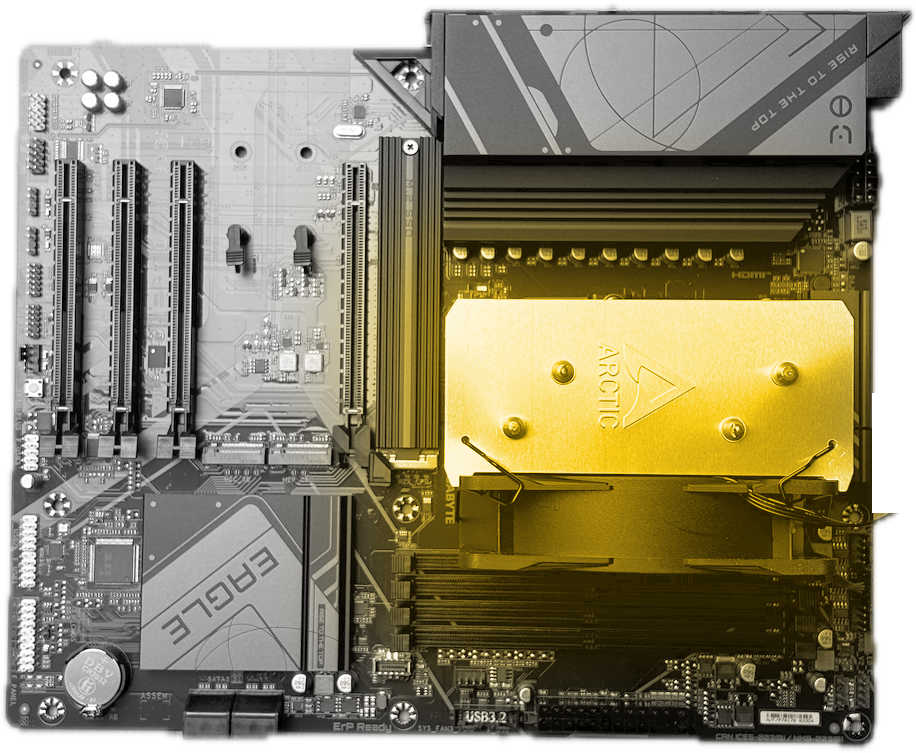
\includegraphics[width=0.45\linewidth]{05_cooler_top_hl}
\caption{AM5 tower air cooler}\label{fig:cooler}
\end{figure}


\newthought{Seat it} by matching the small triangle on the chip's corner to the
triangle on the socket, lower it flat without pressure, close the retention arm
(Figure~\ref{fig:cpu}).




\newthought{Thermal paste}\index{thermal paste} is often pre-applied to the cooler, but if it is not, apply a small pea sized drop to the
    center of the chip, and let the cooler spread it when you mount it.
    Too much paste behaves like a thermal insulator, not a conductor, so don't overdo it at this point.

\newthought{Where the fan plugs in.} The cooler's fan goes on the four
pin header marked \texttt{CPU\_FAN}, right beside the socket. It is the one header
the firmware watches, and a fan anywhere else leaves it reading zero rpm on the
processor, which most boards refuse to boot on.

\marginnote{\newthought{The five fan headers.}\index{fan header} Each is four pin and good for
24~watt.
\begin{itemize}[leftmargin=*, topsep=0.25em, itemsep=0.1em, parsep=0em]
    \item \texttt{CPU\_FAN}: the cooler's fan goes here.
    \item \texttt{CPU\_OPT}: a second CPU fan or pump, right next to it, useful if
    your tower cooler is a dual fan model.
    \item \texttt{SYS\_FAN1}, \texttt{SYS\_FAN2}, \texttt{SYS\_FAN3\_PUMP}: the
    three for the fans you zip tie to the frame rail later.
\end{itemize}}





% ==============================================================================================
% MEMORY
% ==============================================================================================

% No \newpage here: the board section runs long enough that the processor
% subsection breaks on its own, and memory flows onto the page that break opens.
% Memory has to fit that page whole: if its last paragraph spills, storage's
% \newpage below leaves the spill alone on a page of its own. That is why this
% subsection carries no \vspace of its own, and why its prose is cut this tight.
\needspace{9\baselineskip}
\subsection{Memory or RAM}

\newthought{A G.SKILL Ripjaws S5 kit, 64~GB in two 32~GB modules}\index{G.SKILL Ripjaws S5}\index{memory}\index{RAM|see{memory}}, part number
F5-6000J3636F32GX2-RS5K\cite{gskillRipjawsS5}:

\begin{itemize}[topsep=0.25em, itemsep=0.4em, parsep=0em]
    \item RAM kees a weight file warm between loads, plus room
    for the containers layered on later.
    \item For speed the kit runs DDR5-6000\index{memory!DDR5}, double data rate, at CL36-36-36-96\index{memory!CAS latency}
    column address strobe latency and 1.35~volt. Its AMD EXPO profile\index{EXPO profile}, extended
    profiles for overclocking, is where we will take this from in the configuration later on.
    \item We stay at two modules as filling all four slots pushes the memory controller\index{memory!controller}
    down a speed grade.
\end{itemize}

\begin{figure}[!ht]
\centering
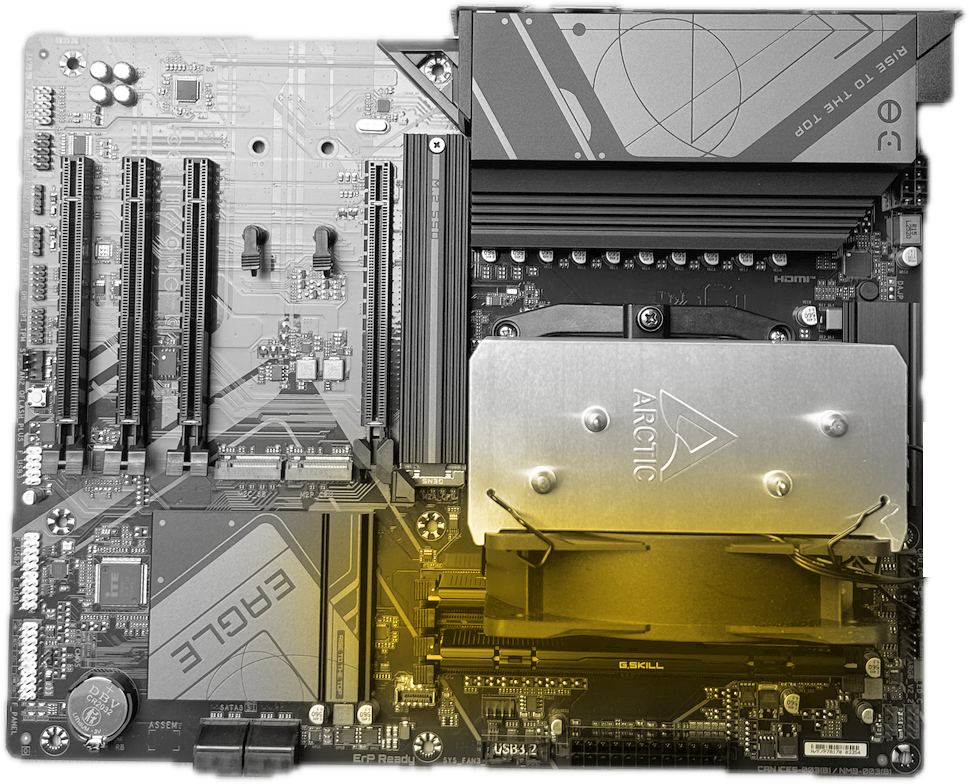
\includegraphics[width=0.45\linewidth]{08_board_populated_hl}
\caption{G.SKILL Ripjaws S5 64\,GB DDR5-6000}\label{fig:memory}
\end{figure}


% Offset pulls the note up beside the bullets. Anchored where it sits, it
% collides with the figure caption that follows, which LaTeX does not warn about.
\marginnote[-4\baselineskip]{\newthought{Why 64 and not 128.} We will be doing fine with 64GB. 
The one real case for a large kit is
offloading a model too big for total VRAM into system memory\index{memory!offloading}, but then again you could just add another 
3090 and have 48GB of VRAM to play with.}

\newthought{Install it} by seating one module in the second slot of each channel\index{memory!channel}, follow the marks on the motherboard or its manual, 
until the clips snap up (Figure~\ref{fig:memory}).





% ==============================================================================================
% STORAGE
% ==============================================================================================

% No \newpage here: storage flows onto the page the memory subsection opened, and
% it puts two items in that margin, its datasheet citation and the capacity note.
% Those two set last on the page, so verify both still render after any edit above.
\needspace{9\baselineskip}
\subsection{Storage}

\newthought{One NVMe drive}\index{NVMe}\index{SSD|see{NVMe}}, for non volatile memory express, 2~TB in the M.2~2280\index{M.2 2280}
size and wired PCIe~4.0~x4, holding both the system and the model library
\cite{gigabyteB650EagleAX}:



\begin{itemize}[topsep=0.25em, itemsep=0.4em, parsep=0em]
    \item For speed it belongs in the first M.2 socket, the only one wired straight
    from the processor. A quantised model\index{quantization} is tens of gigabytes read start to finish
    every time it loads, and that socket is what sets how long we wait on a model swap\index{model swapping}.
    \item For width the socket is PCIe~5.0~x4 while our drive is Gen4~x4\index{PCIe!link width}, so it runs
    at its own full width, around 7.4~GB/s, which is already fast but also leaves headroom left in the socket for a
    faster drive later.
    \item We go for single storage as the second socket runs only PCIe~4.0~x2 and would halve
    this drive's lanes, and the third sits behind the chipset, sharing its uplink
    with network and USB.
\end{itemize}

\begin{figure}[!ht]
\centering
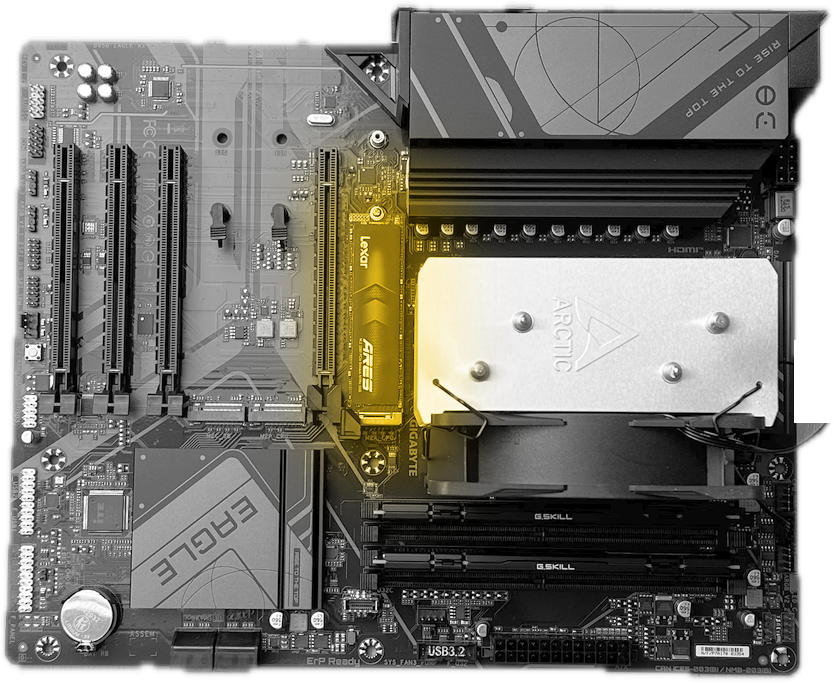
\includegraphics[width=0.45\linewidth]{12_board_complete_hl}
\caption{NVMe Gen4 x4 2\,TB, M.2 2280}\label{fig:nvme}
\end{figure}


% Offset pulls the note up beside the bullets: anchored after the itemize it sets
% level with "Fit the drive" and leaves the whole upper margin empty.
\marginnote[-6\baselineskip]{\newthought{The terabytes are a use-case call}. It leaves
room for a few dozen quantised models\index{model library} beside the system, which is plenty for pure
inference on a handful of models. If you need more models or upgrade regularly pruning will become a housekeeping
chore early one, which is best practice anyway in my opinion.
Datasets, fine tuning\index{fine-tuning} runs and their checkpoints on the other hand quickly will become an issue with 2TB, so size the
drive to what you actually intend to do.}


\newthought{Fit the drive} in the first socket, in at an angle, pressed flat, and
held down with its single screw or latch (Figure~\ref{fig:nvme}).



% ==============================================================================================
% THE FRAME
% ==============================================================================================

\needspace{9\baselineskip}
\section{The Frame}\index{open frame}

\newthought{An open GPU rack frame}. Any aluminium skeleton will do, 
a flat bed for the board and a rail above it
that holds cards upright.

\marginnote{\newthought{Cases are expensive.}\index{case} The downside is that 
the rig is open to dust and to hands, so if you can not move it out of the way - reconsider a case.
Make sure it holds your motherboard and parts in any case. Yep, pun intended.}

\begin{itemize}[topsep=0.25em, itemsep=0.4em, parsep=0em]
    \item For the card, an open bed means it hangs in room air\index{airflow} rather than behind a
    panel, so it runs cooler than the same card in a mid tower.
    \item For growth, the rail makes it easy to swap and add cards easily.
    \item Of course this also gives us a server style look, which I appreciate in this project.
\end{itemize}

\begin{figure}[!ht]
\centering
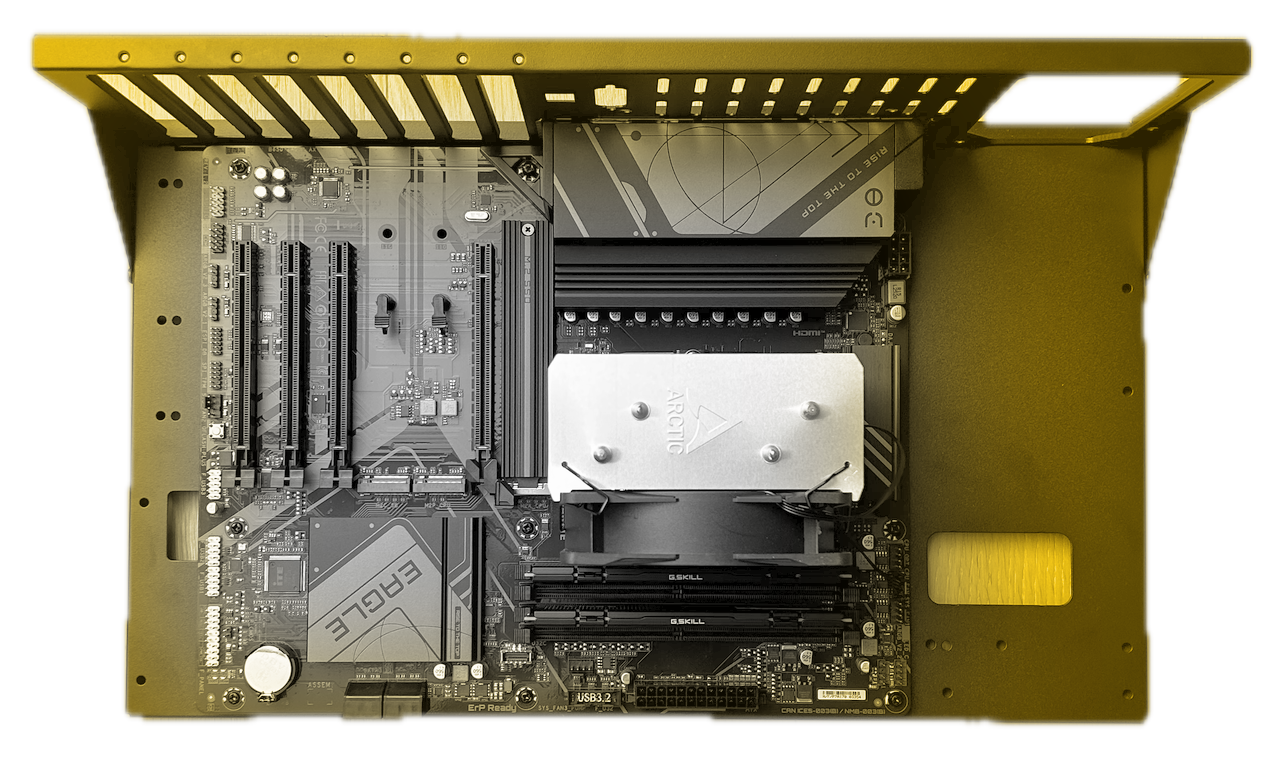
\includegraphics[width=0.77\linewidth]{14_frame_board_mounted_hl}
\caption{Open GPU rack frame}\label{fig:frame}
\end{figure}


\newthought{Mount it now.} Assemble the frame, screw the standoffs\index{standoffs} into the bed, and
lower the populated board onto them. I directly screwed this whole thing into a wall,
but you can also put it on a shelf - if you prefer to not go rogue in your flat. The frame's two pin switch is now 
wired onto \texttt{PW} on \texttt{F\_PANEL}\index{front panel header}.




% ==============================================================================================
% THE GRAPHICS CARD
% ==============================================================================================

\needspace{9\baselineskip}
\section{The Graphics Card}

\marginnote{\newthought{Why the 3090} and not:\index{RTX A6000}
\begin{itemize}[leftmargin=*, topsep=0.25em, itemsep=0.1em, parsep=0em]
    \item A6000, 48~GB: Near ten thousand euro (in 2026).
    \item 5090\index{RTX 5090}, 32~GB: More bandwidth, but no NVLink.
    \item 4090\index{RTX 4090}, 24~GB: The same VRAM at twice the price.
    \item Mac or DGX~Spark\index{DGX Spark}: Unified memory\index{unified memory} crawls on a dense 70~billion parameter
    model.
    \item 3090 Founders Edition\index{Founders Edition}: wants NVIDIA's twelve pin adapter\index{twelve pin adapter} rather than plain
    eight pin cables.
\end{itemize}}

\newthought{A RTX~3090, 24~GB} seated straight in the board's top slot:

\begin{itemize}[topsep=0.25em, itemsep=0.4em, parsep=0em]
    \item For capacity, 24~GB of GDDR6X\index{GDDR6X} VRAM on a 384~bit bus\index{memory!bus width}, which is the limiting factor for model size and
    model context\index{context window}.
    \item For token speed, the 936~GB/s of memory bandwidth\index{memory!bandwidth}\cite{nvidiaRTX3090}
    matters more than the
    10\,496 CUDA cores\index{CUDA cores} while picking a GPU.
    \item For the link, the top slot is the one PCIe~4.0~x16 connection in this
    machine, as long as you go with a single card.
\end{itemize}



\begin{figure}[!ht]
\centering
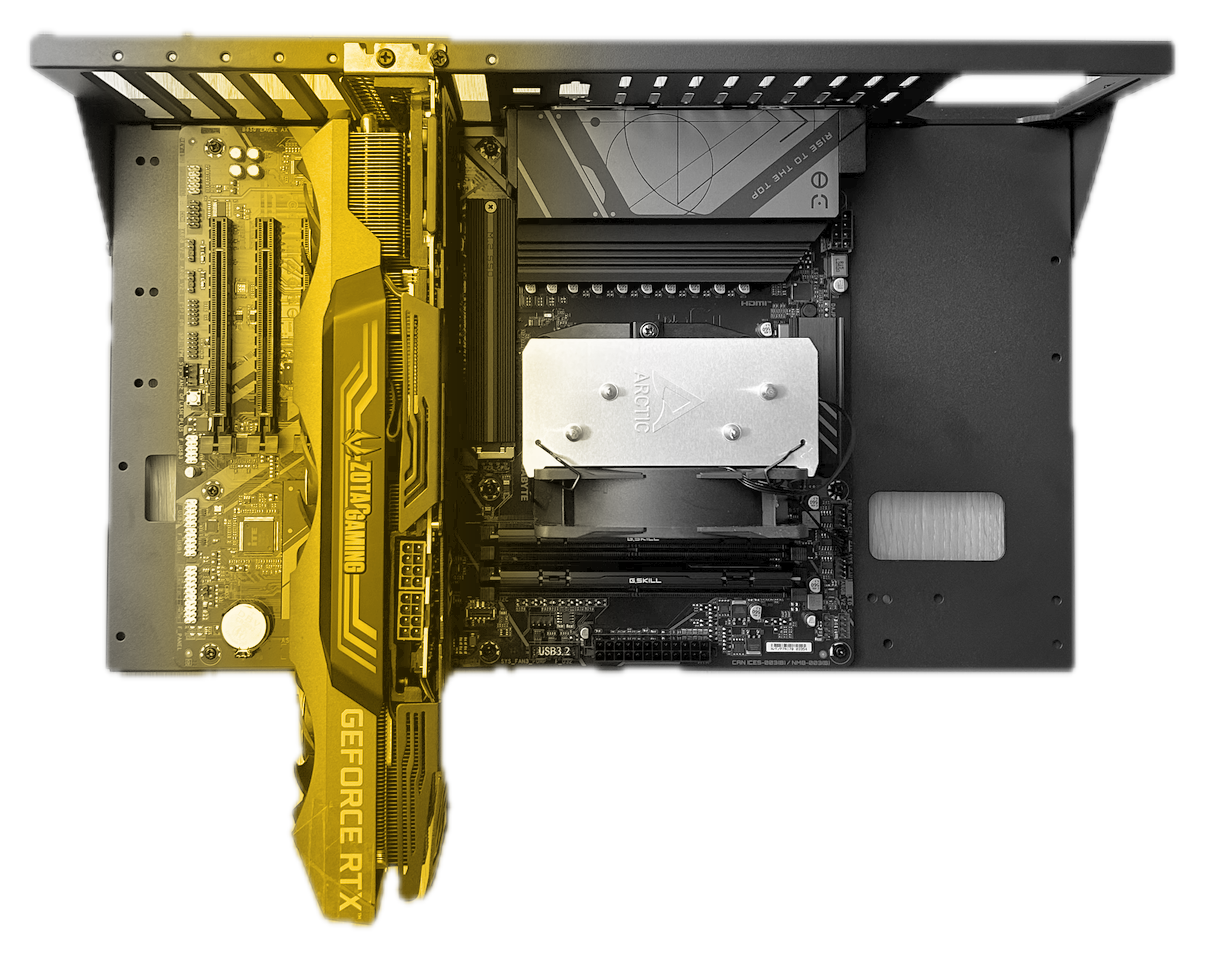
\includegraphics[width=0.75\linewidth]{15_gpu_seated_hl}
% tufte's caption takes [short][offset]; a positive offset lowers it. Sets the
% caption beside the lower part of the card instead of level with its top edge.
\caption[][12\baselineskip]{RTX~3090 24\,GB}\label{fig:gpu}
\end{figure}

\newthought{Fit the card} into the top slot, pressed down evenly until the retention clip snaps shut, fasten its bracket, and leave its power cables until the supply is
mounted. The multi-card rig extensions this motherboard is able to hold will be detailed out in a later section. This in itself is a powerful 
machine.

\marginnote{\newthought{Buying used.}\index{thermal pads}\index{used market} Buy only from a seller who
shows a test of the card under load, and budget a thermal pad replacement. For the used market, a three fan model with two eight pin connectors, an
EVGA FTW3 Ultra, MSI Suprim or Gaming, Gigabyte Gaming~OC, or ASUS~TUF.}

% Placed after the closing paragraph, not after "Fit the card": anchored there its
% caption sets on top of the Buying used marginnote, which LaTeX does not warn about.





% ==============================================================================================
% THE POWER SUPPLY
% ==============================================================================================

\needspace{9\baselineskip}
\section{The Power Supply}

\newthought{An ASRock Phantom Gaming PG-1600G}, 1600~watt against the roughly
500~watt this machine draws, bought for the headroom\index{ASRock PG-1600G}\index{PSU|see{power supply}}\index{power!budget}\cite{asrockPG1600G}:

\marginnote{\newthought{Get solar power for your idle wattage.}\index{Balkonkraftwerk}\index{solar power}\index{power!idle draw}
The floor runs day and night whether or not anyone prompts the machine, and most of it
is the platform rather than the card. A steady draw is what a balcony solar setup
covers best: panels and a capped inverter suit a constant load, not the spikes this
supply was bought to survive. Put a meter\index{power meter} on the wall socket before sizing any of it.}

\begin{itemize}[topsep=0.25em, itemsep=0.4em, parsep=0em]
    \item For the graphics card, a 3090 averages 350~watt and spikes far above it,
    which is what trips undersized supplies mid run\index{power!transient spikes}. ATX~3.1\index{ATX 3.1} rates this unit for
    220 percent of that, and the 1600~watt rating is what we need for four potential cards.
    \item For the board, one 24~pin main cable\index{ATX 24 pin} and one processor cable, 4+4~pin,
    both modular\index{modular cables}, so only what we use leaves the unit.
    \item Eight PCIe cables\index{PCIe!power cable} ship in the box. We wire two, and the rest is already
    there for later cards.
\end{itemize}

\begin{figure}[!ht]
\centering
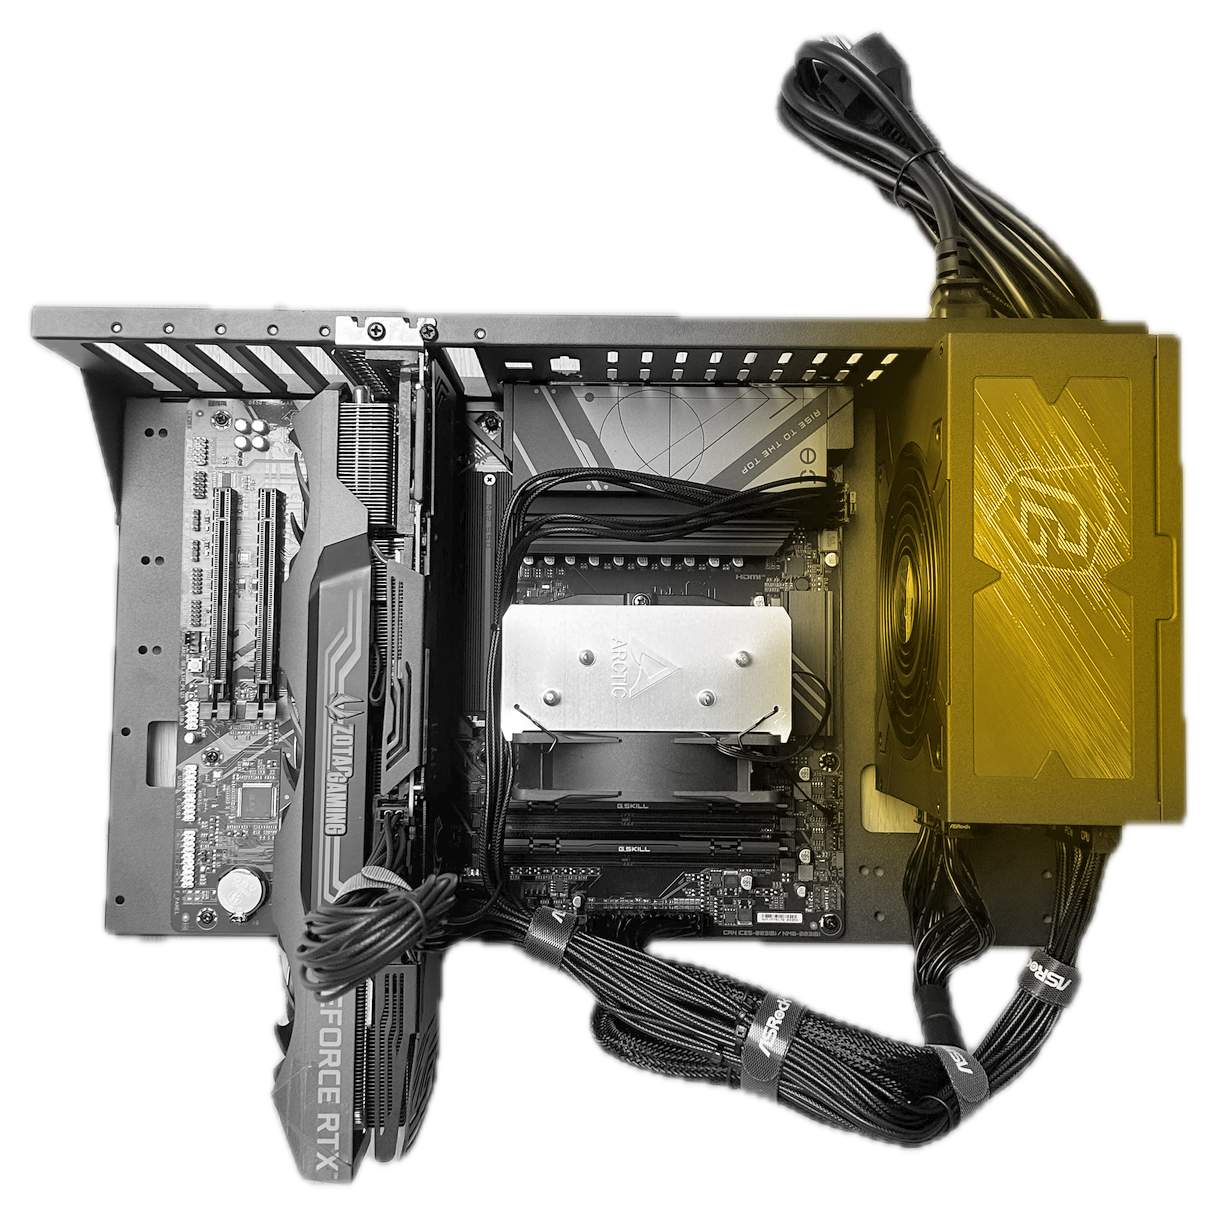
\includegraphics[width=0.81\linewidth]{19_psu_mounted_hl}
\caption{ASRock PG-1600G, 1600\,W}\label{fig:psu}
\end{figure}


\marginnote{\newthought{What stays in the box.} The unit ships two processor cables
and this board takes one, so there is no second socket to hunt for. The two 12V-2x6\index{12V-2x6}
cables, 600~watt each, are for 40 and 50 series cards, while a 3090 takes plain eight
pin. Twelve SATA\index{SATA power} and six Molex\index{Molex} wait for spinning storage or a powered riser.}

\newthought{Wire it last.} Mount the supply on the frame, then run the cables in this
order:

\begin{enumerate}[topsep=0.25em, itemsep=0.4em, parsep=0em]
    \item The 24~pin main cable (often it is labelled MB) into \texttt{ATX}, the widest socket on the board,
    sitting on the long edge alongside the memory slots. Press until the latch clicks.
    \item The 4+4~pin processor cable, from the socket marked \texttt{CPU} on the
    supply into \texttt{ATX\_12V}\index{ATX 12V} on the board, on the short edge past the cooler,
    beside the VRM\index{VRM} heatsink nearest the rear I/O panel.
    \item The two PCIe cables to the card's own two eight pin connectors\index{eight pin connector}, along its
    top edge, one cable each and never daisy chained\index{daisy chaining}.
\end{enumerate}



\newthought{Leave the mains lead unplugged.} The rig is now fully assembled, wired, and ready to be powered on for the first time.
Skip to \hyperref[ch:engine]{the next chapter} for the firmware setup and the first
probe of the rig.









% ==============================================================================================
% CARDS TWO TO FOUR
% ==============================================================================================

\newpage
\section{Multi-Card Rig}\index{multi-card rig}

\newthought{One to three more RTX~3090s} find a place on this rig
design\cite{gigabyteB650EagleAX}. A second card
buys memory for larger models, while the third and fourth cards buy additional throughput.

\needspace{9\baselineskip}
\subsection{Card Two}\index{NVLink}

\marginnote{\newthought{What NVLink is.} A bridge that clips onto the top edge of
two cards and carries 112.5~GB/s bidirectional traffic on
the 3090.}

\newthought{Stay on the 3090.} It is the only GeForce~30 card
with NVLink, so a matched pair takes a bridge and pools\index{memory!pooling} to 48~GB for one model. 
Mixed cards never pool.

\newthought{The rest is mechanical.} Drop the card into the next x16 sized
position, wired PCIe~3.0~x1, on a plain riser\index{riser}\index{mining}. 
Riser spacing is yours to set, so match it to
the bridge you buy, get it fixed on your frame, and run its own two cables from the supply.

\needspace{9\baselineskip}
\subsection{Cards Three and Four}

\newthought{Add these with increased workload.} Two x16 sized positions remain, one
from the processor and one from the chipset. Both are wired PCIe~3.0~x1\index{PCIe!x1 lane}: full length
connector, a single lane\index{PCIe!lanes} behind it, about 1~GB/s only.
Keep it at one model per (linked) card(s). A model split across cards
parallelism\index{tensor parallelism} moves activations every token and starts to crawl. So the idea is to have the same model loaded
    on each card, and let the engine\index{engine} round robin\index{round robin} between them for throughput.

\marginnote{\newthought{On power.} Four cards at 350~watt plus the
platform reach roughly 1550~watt, which becomes uncomfortable against our supply's 1600 limit.
Undervolted\index{undervolting} near 0.875~volt each card draws about 280 and the whole rig lands near
1270, which makes it comfortable again.}

\newthought{4 Cards will definitely get you Fans.} Zip tie a bank of case
fans\index{case fans} along the rail, undervolt before the fourth cars goes in.



% ==============================================================================================
% THE MINIMAL VIABLE RIG
% ==============================================================================================

% The second thread, for a reader who wants every step of this book without the
% silicon. Same three newthought shape as a part section, same scope rule: it stops
% at the assembled, unpowered board. Everything above the metal is identical, which
% is the whole argument, and it lives in the margin rather than the main column.
\newpage
\section{The Minimal Viable Rig}\index{Raspberry Pi}\index{LPDDR4X}

\newthought{A Raspberry Pi~5 with 8~GB}, (go 16 GB if you can) an active cooler\index{active cooler}, the official
5~volt 5~amp USB-C supply\index{USB-C power} and a 64~GB microSD card\index{microSD}\cite{raspberrypiPi5}, 
will enable you to learn just as much on a tighter budget.

\marginnote{\newthought{The On-A-Budget-Thread.} Same operating system, same
container runtime, same engine binary on the same port, same clients pointed at it.
Only the model and performance shrinks.}

\newthought{The 8~GB is shared}\index{unified memory}: processor and graphics core read the same
LPDDR4X, so it is system and video memory at once. A four billion parameter model at
four bit quantisation\index{quantization} takes near 2.5~GB and leaves five for the operating system and
containers. What it costs mainly is speed as 
LPDDR4X-4267 moves roughly 17~GB/s\index{memory!bandwidth} where a 3090 moves 936, and generation reads
the whole model once per token, so answers arrive at single digit tokens per
second\index{tokens per second} rather than dozens. But hey we don't care about speed for learning, 
and buying hardware later on is the easy part.

\newthought{Build it in five minutes.} Clip the active cooler onto the board and plug
its fan into the header beside it, write the operating system image onto the microSD
card and seat the card in the slot on the underside, and leave the USB-C supply out of
the wall. A complete machine, wired and never switched on, in one hand.


% ==============================================================================================
% BRIDGE
% ==============================================================================================
\vfill
\newthought{The metal is finished}, whichever of the two machines is on
your bench. What it still lacks is a first power on and a handful of firmware values
that make a card addressable, a probe that proves every part is really on the bus,
and then an operating system, a driver, and weights loaded into memory together with some orchestration. 
Let's get on it.


% CHAPTER 2: the engine, first boot, OS, driver, Docker, Ollama, Open WebUI
%% !TEX root = ../notes_sovereignai.tex
% Chapter 2: The Engine. First boot, OS, driver, Docker, Ollama, Open WebUI.
%
% This chapter owns everything from the first power-on onward. Firmware setup and
% the enumeration probe live here, not in the hardware chapter: they are the first
% thing software does to the rig, and they are what separates a hardware fault from
% a software one before there is any software to blame.
%%%%%%%%%%%%%%%%%%%%%%%%%%%%%%%%%%%%%%%%%%%%%%%%%%%%%%%%%%%%%%%%%%%%%%

\index{Ollama}\index{Open WebUI}\index{Docker}\index{CUDA}\index{Ubuntu Server}\index{NVIDIA driver}
\chapter{The Engine}
\label{ch:engine}
\printchapterversion{02_engine}
\newthought{Silicon, Meet Software.}
\vspace{1.5em}

% ==============================================================================================
% THE WHY
% ==============================================================================================

\section{The Why}\index{inference}\index{container runtime}

\newthought{The rig is assembled}, wired, and has never been switched on. A graphics card is
only potential until software puts a model on it and hands you a way to ask
questions. This chapter powers the machine for the first time, proves every part
is really there, and turns the metal into a served model the whole family can talk
to, with the least machinery that works: firmware, an operating system, a driver, a
container runtime, and one program that loads models onto the GPU.

\newthought{That program is Ollama.}\index{Ollama!install} It is the shortest path to local
inference: one command installs it, it finds the GPU on its own, and it serves an
API\index{OpenAI-compatible API} the rest of the world already speaks. In front of it we put
Open WebUI, a private chat in the browser, so the family has something to use on
day one and you have an account system to build on later.

\marginnote{\newthought{Why not vLLM yet.}\index{vLLM} vLLM wins when many people hit the
box at once, and it is also what answers a narrow slot: cards two to four sit on a
single PCIe lane, where tensor parallelism\index{tensor parallelism} would push activations across the
link on every token. vLLM need not split a model that way. A replica per card, or a
split by layer with pipeline parallelism\index{pipeline parallelism}, sends almost nothing over the link,
so lane width stops mattering and the answer stays in software rather than in a
server board. On one card serving a household, Ollama's one command beats vLLM's
tuning, and both speak the same OpenAI-compatible API, so the swap is later and cheap.}

\newthought{By the end of this chapter} you will have:
\begin{itemize}
    \item set five firmware values and proved the hardware enumerates before an
    operating system touched the drives;
    \item put Ubuntu Server, the NVIDIA driver, and GPU-aware Docker on the rig;
    \item run a model on the 3090 with Ollama and confirmed it answers on the API;
    \item stood up Open WebUI and chatted with the model from a browser on your LAN.
\end{itemize}

% ==============================================================================================
% FIRST BOOT
% ==============================================================================================

\section{First Boot}\index{firmware}

\newthought{Power on.} Connect the monitor to the board's own display output, not to
the graphics card, switch the supply on, and press the power button. The fans should
spin up and hold; a half turn and a stop means the supply or the 24~pin is not
seated. Enter setup when the splash appears.

\marginnote{\newthought{Two of these are for later.} Above 4G Decoding and
Resizable BAR only bite once a second card arrives, so set them now, while the
rail is still empty and a later card cannot fail in a way that looks like dead
hardware.}

\newthought{Set five values}\index{Above 4G Decoding}\index{Resizable BAR}\index{IOMMU}\index{integrated graphics}\index{EXPO profile}\index{XMP profile}, then save and exit:

\begin{verbatim}
Above 4G Decoding ............ Enabled
Re-Size BAR Support .......... Enabled
IOMMU ........................ Enabled
Initial Display Output ....... IGD
EXPO / XMP profile ........... Profile 1
\end{verbatim}

\marginnote{\newthought{What they do.} Above 4G Decoding gives the cards address
space beyond the 32~bit boundary, without which a second card fails to map at all.\index{VRAM}
Resizable BAR lets the processor address a card's whole VRAM in one window, which
speeds weight loading. IOMMU keeps device passthrough\index{device passthrough} available. Initial Display
Output on the integrated graphics leaves all 24~GB of every card free for models.}

\newthought{The last of the five is the memory.} A DDR5 kit does not run at the
speed on its box until you say so: leave the EXPO profile off and the modules clock
themselves to the conservative default published by JEDEC\index{JEDEC}, the memory standards
body, rather than the rated 6000 they were bought for. This is the one firmware
value that changes nothing about whether the machine works and everything about how
fast it feeds the cards.

\marginnote{\newthought{Menu names move.} These five sit under different headings
in different firmware revisions of the same board. Use the setup search rather than
trusting a path from a screenshot, and set all five in one visit: a value missed
here surfaces later as a hardware fault that is not one.}

\newthought{Probe before you install anything.}\index{lspci}\index{enumeration} Boot an Ubuntu Server image from a
USB stick and choose to try it without installing. Nothing here writes to the
drives:

\begin{verbatim}
$ lscpu | grep 'Model name'   # AMD Ryzen 5 9600X
$ free -h                     # total ~ 62Gi
$ lspci | grep -i nvidia      # NVIDIA GA102 [RTX 3090]
$ lspci -vv | grep LnkSta:    # Width x16
\end{verbatim}

\marginnote{\newthought{Why this proves anything.} Enumeration is the firmware
naming each device on the bus, and it happens with no driver loaded. A card that
enumerates is seated, powered, and addressable, which separates a hardware fault
from a software one before there is any software to blame.}

\newthought{Four clean answers} clear the way for software: the right processor, the
full memory, an NVIDIA device on the bus, and that device at x16. If the card is
missing, reseat the riser and confirm both eight pin cables. If the width reads x1,
the card is on the wrong slot or the wrong riser. If memory reads half, reseat the
second module. Past this point every failure is a software failure.

\marginnote{\newthought{Link speed, read honestly.}\index{PCIe!link width} \texttt{LnkSta} is the
negotiated state, not the capability, and a card at idle may report a lower speed
until it is put to work. Width is the number to trust here.}

% ==============================================================================================
% LOCAL SERVING
% ==============================================================================================

\section{Local Serving}\index{quantization}\index{model weights}

\newthought{A served model is a stack} four layers deep. The operating system
owns the hardware; the NVIDIA driver\index{NVIDIA driver} lets programs reach the card; the NVIDIA
Container Toolkit\index{NVIDIA Container Toolkit} lets Docker containers reach it too, so every service in this
book ships as a container without fighting over the GPU; and Ollama sits on top,
loading model weights\index{model weights} into the 24~GB of video memory\index{VRAM} and answering requests.

\marginnote{\newthought{Why containers.} Each later service, the chat, the voice
pipeline, image generation, is a container that asks Docker for the GPU\index{Docker!GPU passthrough} and gets
it. The toolkit passes the host driver through, so you install the driver once on
the metal and never again inside a container.}

\newthought{Models come quantized.} A model's weights are shrunk from sixteen bit
floats to four or five bits with little loss\index{quantization}, which is what lets a capable model
fit in 24~GB. Ollama pulls these as ready-to-run files and picks a sensible
quantization for you; a fourteen billion parameter model leaves headroom for
context, a thirty billion parameter mixture-of-experts\index{mixture of experts} model fills the card and is
the ceiling for a single 3090.

\marginnote{\newthought{Pick a tool-caller.}\index{tool calling} Choose from the Qwen3\index{Qwen3} family. Beyond
chat quality, prefer a model that supports tool calling, since Chapter~4's voice
assistant cannot flip a single switch without it. Filter the model library by
\texttt{tools} and ignore the rest.}

\newthought{The API is the point.}\index{Ollama!API} Ollama serves an OpenAI-compatible endpoint at
\texttt{:11434/v1}, the same shape every client in this book speaks. Two cautions
that Chapter~3 acts on: it binds to localhost and it has no authentication, so on
its own it is reachable only from the machine itself, and opening it to the
network without a gateway in front would leave it wide open\cite{ollamaDocs}.

\section{Run a Model}\index{nvidia-smi}

\marginnote{\newthought{Headless is the habit.}\index{SSH} Do all of this over SSH from your
laptop; the rig needs no monitor of its own. Run the GPU steps first, because every
later one assumes the card is visible to software.}

\newthought{Lay the foundation.}\index{Ubuntu Server} Install Ubuntu Server~24.04 from the same USB
stick you probed with, then the driver and a GPU-aware Docker:

\begin{verbatim}
$ sudo ubuntu-drivers install          # NVIDIA driver
$ sudo reboot
$ nvidia-smi                           # the 3090 appears, with its 24 GiB

$ curl -fsSL https://get.docker.com | sh
$ sudo nvidia-ctk runtime configure --runtime=docker
$ sudo systemctl restart docker
$ docker run --rm --gpus all ubuntu nvidia-smi   # the card, now inside a container
\end{verbatim}

\marginnote{\newthought{Split the drive here, not at the shop.}\index{partitioning}\index{Ollama!model directory} Manual partitioning
in the installer gives the system its own partition and leaves the rest as a
separate filesystem for weights, and the board keeps two free M.2 sockets if a
second drive comes later. Either way \texttt{OLLAMA\_MODELS} points at the large
volume, so reinstalling the operating system never touches a model library that
took days to download.}

\newthought{Install the engine and pull a model.}\index{Ollama!model pull}\index{model library} One command installs Ollama,
which detects the card; one more pulls a model and opens a chat:

\begin{verbatim}
$ curl -fsSL https://ollama.com/install.sh | sh
$ ollama pull qwen3:14b
$ ollama run qwen3:14b      # type a question; watch nvidia-smi load the card
\end{verbatim}

\newthought{Confirm it answers on the API}, the interface every later chapter
uses:

\begin{verbatim}
$ curl http://localhost:11434/v1/chat/completions -d '{
    "model": "qwen3:14b",
    "messages": [{"role": "user", "content": "say hello"}]
  }'
\end{verbatim}

\newthought{Put a face on it.}\index{Docker!volume} Run Open WebUI as a container pointed at Ollama,
with a named volume so accounts and history survive restarts:

\begin{verbatim}
$ docker run -d --name open-webui -p 3000:8080 \
    --add-host=host.docker.internal:host-gateway \
    -e OLLAMA_BASE_URL=http://host.docker.internal:11434 \
    -v open-webui:/app/backend/data \
    ghcr.io/open-webui/open-webui:main
\end{verbatim}

\marginnote{\newthought{The first account is admin.}\index{Open WebUI!accounts} Open WebUI's first sign-up
becomes the administrator; create it, then add an account for each member of the
household under the admin panel. That account system is the gateway Chapter~3 hands
keys from.}

\newthought{What you now own} is a served model. From any browser on your home
network, open \texttt{http://rig-address:3000}, sign in, and chat. A family member
two rooms away is talking to a model running on your 3090, with no token metered
and no prompt leaving the house.

% ==============================================================================================
% BRIDGE
% ==============================================================================================

\newthought{The engine runs, but only at home.} It answers on the local network and
nowhere else, and it trusts anyone who can reach it. The next chapter carries it to
your phone, your laptop, and your terminal wherever they are, without opening the
box to everyone.

\marginnote{\newthought{feedback}}


% CHAPTER 3: everywhere, Tailscale / Cloudflare exposure + Open WebUI API keys
%% !TEX root = ../notes_sovereignai.tex
% Chapter 3: Everywhere. Tailscale mesh, the tailnet as the credential.
% Ollama leaves the box here, and nothing else does: the browser chat and
% the family door belong to the chapter after this one, because they are ways
% of reaching it rather than ways of carrying it.
%%%%%%%%%%%%%%%%%%%%%%%%%%%%%%%%%%%%%%%%%%%%%%%%%%%%%%%%%%%%%%%%%%%%%%

\index{Tailscale}\index{API key}\index{tailnet}\index{device identity}
\chapter{Everywhere}
\printchapterversion{03_everywhere}
\newthought{Reachable, Not Exposed.}
\vspace{1.5em}

% ==============================================================================================
% THE WHY
% ==============================================================================================

\section{The Why}\index{remote access}\index{attack surface}

\newthought{Ollama answers on the machine itself} and nowhere else. That is fine
for a terminal on the rig and useless for the rest of life: the laptop on a train,
the phone in another country, the coding agent in your terminal at work. This
chapter carries its API to those devices without carrying it to anyone else.

\marginnote{\newthought{Reach and proof are one job here.} Getting a request from a
foreign network to your card is one problem, and proving the request came from you
is another. A mesh answers both at once, because a device that cannot join cannot
send, which is why nothing in this chapter issues a password.}

\newthought{The danger to respect} is that Ollama has no password and was built to
listen only to its own machine. The lazy fix, binding it to the network directly,
hands your GPU to the internet\index{port forwarding}: an open \texttt{11434} is a model
anyone can run at your electricity bill's expense, and a prompt log they can read.
So nothing is exposed raw. A private mesh carries you to the box instead, and
membership of that mesh is the credential.

\newthought{By the end of this chapter} you will have:
\begin{itemize}
    \item joined the rig to a private mesh and reached it by name from a foreign network;
    \item served Ollama over HTTPS on that mesh, with no port forwarded;
    \item driven it from a terminal coding agent off-site through two environment variables.
\end{itemize}

% ==============================================================================================
% REACH AND AUTH
% ==============================================================================================

\section{Reach and Auth}\index{mesh VPN}\index{tunnel}\index{authentication}

\newthought{Tailscale} builds a private encrypted mesh between your own devices.
Install it on the rig and on your laptop and phone, and they reach each other by a
stable name as if on one LAN, through firewalls and carrier NAT\index{NAT traversal}, with no port
forwarded and nothing published. The tailnet itself is the authentication: only
your enrolled devices\index{tailnet} can connect, so the box is reachable everywhere by you and
invisible to everyone else\cite{tailscaleSelfHostAI}.

\marginnote{\newthought{Mesh versus tunnel.}\index{Cloudflare!Tunnel} A mesh joins devices you
own into one private network, and it is the whole of this chapter. A tunnel
publishes one service to the public web behind a login, which is what a relative
who will not install a VPN needs and what a raw model API must never be.
Publishing waits until there is a page worth publishing.}

\newthought{The mesh carries the key field with it.}\index{API key!placeholder} A client still
sends an authorisation header, and Ollama still ignores it, so the credential
is the device rather than the string. That is a stronger claim than it sounds:
a leaked key is a key someone else can use, and a leaked tailnet name is a name
that resolves for nobody. What it costs is that every client must be a device you
enrolled, which is the point.

\marginnote{\newthought{When the client cannot join.}\index{bearer token}\index{reverse proxy} A build server or a
shared box you do not own cannot run Tailscale, and then the device stops being
the credential. Put a reverse proxy in front of \texttt{11434} that requires a
bearer token\index{coding agent} and forwards only on a match, and the token becomes the
credential for that one client. Every device you do own stays on the mesh.}

% ==============================================================================================
% USE IT ANYWHERE
% ==============================================================================================

\section{Use It Anywhere}\index{tailscale serve}\index{Tailscale}

\marginnote{\newthought{Install once per device.} Tailscale goes on the rig and on
every device you want to reach it from. The phone and laptop apps are a login, not a
config file.}

\newthought{Join the rig to your mesh}, then reach it by name:

\begin{verbatim}
$ curl -fsSL https://tailscale.com/install.sh | sh
$ sudo tailscale up                    # log in once in the browser
$ tailscale serve --bg 11434           # Ollama over HTTPS on the tailnet
\end{verbatim}

\newthought{Reach it from anywhere.} With Tailscale running on your laptop, the rig
answers at its tailnet name over HTTPS, on cellular, in another country, with
nothing exposed to the public internet and no port forwarded on your router.

\newthought{Point a program at it} with two environment variables, which is the
whole of the client setup for anything that speaks the OpenAI shape:

\begin{verbatim}
$ export OPENAI_API_BASE=https://rig.your-tailnet.ts.net/v1
$ export OPENAI_API_KEY=ollama         # the mesh is the credential
$ curl $OPENAI_API_BASE/chat/completions \
    -H "Authorization: Bearer $OPENAI_API_KEY" \
    -d '{"model":"qwen3.8:27b","messages":[{"role":"user","content":"hi"}]}'
\end{verbatim}

\marginnote{\newthought{Coding agents.} Aider, OpenCode, and Cline all take an
OpenAI base URL and key, so the two variables above are the whole setup. Even Claude
Code can be pointed home with \texttt{ANTHROPIC\_BASE\_URL} set to the same host and
\texttt{ANTHROPIC\_AUTH\_TOKEN} set to any string.}

\newthought{What you now own} travels with you. From a laptop on a foreign network,
your terminal coding agent reads the two variables, sends a task to the rig at home,
and edits your code on a model nobody meters.

% ==============================================================================================
% BRIDGE
% ==============================================================================================

\newthought{Ollama is now everywhere you type}, on every device you own and on
no device you do not. What it still lacks is a face: reaching it means a terminal
and a curl, which is no way to hand a model to the rest of the household. The next
chapter gives it a screen anyone can open and a voice that answers out loud,
without a word leaving the building.

\marginnote{\newthought{feedback}}


% CHAPTER 4: a voice in the house, Home Assistant + Wyoming + Whisper + Piper + Ollama
%% !TEX root = ../notes_sovereignai.tex
% Chapter 4: A Voice in the House. HA + Wyoming + Whisper + Piper + Ollama.
%%%%%%%%%%%%%%%%%%%%%%%%%%%%%%%%%%%%%%%%%%%%%%%%%%%%%%%%%%%%%%%%%%%%%%

\index{Home Assistant}\index{Wyoming}\index{Whisper}\index{Piper}\index{voice assistant}
\chapter{A Voice in the House}
\printchapterversion{04_voice}
\newthought{Speak, and It Answers.}
\vspace{1.5em}

% ==============================================================================================
% THE WHY
% ==============================================================================================

\section{The Why}\index{smart home}\index{privacy}

\newthought{The engine reaches every screen you own} and none of the air in the room. A voice
assistant closes that gap, and it is the one piece of household AI most people
already rent in its worst form: an always-listening microphone that ships every
word to a company's servers. The sovereign version hears, thinks, and speaks
entirely on your hardware, and it can act on the house rather than only answer
trivia.

\newthought{The orchestrator is Home Assistant.}\index{Home Assistant!container} It is the open hub the smart-home
world already speaks, it runs as a container on the rig, and its voice pipeline is
built from swappable parts joined by a small protocol. We give it a local ear, a
local voice, and the local model as its brain.

\newthought{By the end of this chapter} you will have:
\begin{itemize}
    \item run Home Assistant with local speech-to-text and text-to-speech;
    \item made the Ollama model its conversation brain, able to act on devices;
    \item spoken to a satellite and heard the rig answer, with nothing leaving the house.
\end{itemize}

% ==============================================================================================
% SPEECH TO MODEL TO SPEECH
% ==============================================================================================

\section{Speech to Model to Speech}\index{speech to text}\index{text to speech}%
\index{STT|see{speech to text}}\index{TTS|see{text to speech}}

\newthought{A voice turn is three steps.} Speech-to-text turns the spoken request
into words; the model decides what it means and what to do; text-to-speech turns
the answer back into sound. The local stack is faster-whisper for the ear, the
Chapter~2 model for the brain, and Piper for the voice, each a small service, each
replaceable.

\marginnote{\newthought{Wyoming}\index{Wyoming!protocol} is Home Assistant's protocol for voice parts: each
service listens on a TCP port and speaks audio and events, and Home Assistant wires
them into a pipeline. Whisper listens on \texttt{10300}, Piper on \texttt{10200}.}

\newthought{Put the ear on the GPU.}\index{faster-whisper} Speech-to-text is the slow step, and the
built-in add-on runs on the CPU; running faster-whisper as its own container with
the GPU passed through brings a request under a second. The same 3090 that serves
chat transcribes speech in the gaps, since the two rarely peak at once in a house.

\marginnote{\newthought{The brain must hold tools.}\index{tool calling}\index{conversation agent} A conversation agent that only
chats can answer the weather but cannot turn off a light. Home Assistant exposes its
devices to the model as tools, so the model must be one that supports tool calling;
the Qwen3 model from Chapter~2 was chosen for exactly this.}

% ==============================================================================================
% WIRE THE PIPELINE
% ==============================================================================================

\section{Wire the Pipeline}\index{voice pipeline}

\newthought{Run the orchestrator and the voice parts} as containers on the rig:
Home Assistant, the ear with the GPU passed through, and the voice.

\begin{verbatim}
$ docker run -d --name homeassistant --network host \
    -v ha-config:/config ghcr.io/home-assistant/home-assistant:stable

$ docker run -d --name whisper -p 10300:10300 --gpus all \
    rhasspy/wyoming-whisper --model small-int8 --language en --device cuda

$ docker run -d --name piper -p 10200:10200 \
    rhasspy/wyoming-piper --voice en_US-lessac-medium
\end{verbatim}

\marginnote{\newthought{Add the parts in the UI.}\index{Home Assistant!Wyoming integration} In Home Assistant, Settings,
Devices and Services, add the Wyoming Protocol integration twice, pointing it
at the rig's address on ports \texttt{10300} and \texttt{10200} to register the ear
and the voice.}

\newthought{Make the model the brain.}\index{Home Assistant!Ollama integration} Add the Ollama integration and point it at
the engine, then choose a tool-calling model:

\begin{verbatim}
Settings > Devices & Services > Add Integration > Ollama
  URL ..... http://localhost:11434
  Model ... qwen3:14b
  [x] let the model control Home Assistant devices
\end{verbatim}

\newthought{Assemble the pipeline.}\index{Home Assistant!voice pipeline} Under Settings, Voice Assistants, build one
assistant from the three local parts: faster-whisper for speech-to-text, the Ollama
agent for conversation, and Piper for text-to-speech. Set it as the preferred
assistant.

\marginnote{\newthought{Give it ears in a room.}\index{voice satellite}\index{Wyoming!satellite} A Home Assistant Voice PE puck, or
any Wyoming satellite, is the microphone and speaker on the shelf; it hands audio to
the pipeline and plays the answer back. One per room you want to talk to.}

\newthought{What you now own} answers out loud. You say ``turn off the kitchen light
and tell me a joke.''
The satellite streams it to the rig, faster-whisper transcribes it, the model turns
off the light through Home Assistant and writes a reply, and Piper says it back, all
on hardware you own, with the router unplugged if you like.

% ==============================================================================================
% BRIDGE
% ==============================================================================================

\newthought{The house can now listen and speak}, and chat, terminal, and voice all
draw on the one engine. What the engine still lacks is your own life: it answers
from what it was trained on, never from what you have written. The next chapter
points your notes at it.

\marginnote{\newthought{feedback}}


% CHAPTER 5: second brain, Obsidian on the local engine
%% !TEX root = ../notes_sovereignai.tex
% Chapter 5: Second Brain. Obsidian on the local engine.
%%%%%%%%%%%%%%%%%%%%%%%%%%%%%%%%%%%%%%%%%%%%%%%%%%%%%%%%%%%%%%%%%%%%%%

\index{Obsidian}\index{embeddings}\index{retrieval}\index{second brain}\index{markdown}
\chapter{Second Brain}
\printchapterversion{05_secondbrain}
\newthought{Chat With What You Know.}
\vspace{1.5em}

% ==============================================================================================
% THE WHY
% ==============================================================================================

\section{The Why}\index{retrieval augmented generation}\index{RAG|see{retrieval augmented generation}}

\newthought{The model answers from what it was trained on}, not from what you have lived. It has
never read your meeting notes, your reading highlights, the half-finished thoughts in
your vault. Point your notes at the engine and it answers from your own record
rather than from general knowledge, while the notes themselves never leave your
machine.

\marginnote{\newthought{Obsidian}\index{Obsidian!vault} keeps a vault as plain markdown files in a folder
on your own disk, with no server and no account behind it, which is what makes a
private path from the vault to the engine a matter of pointing a plugin at an
address.}

\newthought{The tool is Obsidian} with two community plugins\index{Obsidian!plugins}: one to chat with the
vault, one to find related notes by meaning. Both point at the Chapter~2 engine over
the private network from Chapter~3, so a question typed on your laptop is answered by
the rig at home, grounded in your writing.

\newthought{By the end of this chapter} you will have:
\begin{itemize}
    \item pulled an embedding model and exposed it through the engine;
    \item connected Obsidian's chat and semantic-search plugins to the rig;
    \item asked a question and received an answer drawn from your own notes.
\end{itemize}

% ==============================================================================================
% NOTES AS CONTEXT
% ==============================================================================================

\section{Notes as Context}\index{embedding model}\index{semantic search}\index{context window}

\newthought{A model reads only its prompt.} To answer from your notes, the relevant
notes must be found and placed into the prompt before the model runs. That is
retrieval-augmented generation\index{retrieval augmented generation}: search the vault for what bears on the question, hand
those passages to the model as context, and let it answer over them. The model is not
retrained; it is briefed.

\marginnote{\newthought{Embeddings}\index{vector} turn each note into a vector, a point in meaning
space, so that notes about the same idea land near each other even when they share no
words. A question becomes a vector too, and the nearest notes are its answer's
sources. This is what makes search find sense, not just strings.}

\newthought{Two models, two jobs.} Search needs an embedding model, small and fast,
that vectorises every note once and the question each time; answering needs the chat
model from Chapter~2. Both run on the rig through Ollama, so the embedding model is a
one-line pull and the vault is indexed against your own hardware.

\marginnote{\newthought{Already partly solved.}\index{knowledge base} Open WebUI carries its own retrieval:
drop a PDF or a folder into its knowledge feature and it embeds and searches them the
same way. Obsidian is the version that lives inside your notes;
the next chapter points at the broader cases.}

\newthought{Where the work runs.}\index{tailnet} Obsidian runs on your laptop, the engine on the
rig. The plugins reach the engine at its address on your tailnet, so indexing and
chat happen on the 3090 while the vault stays on the laptop, and nothing crosses the
public internet.

% ==============================================================================================
% WIRE OBSIDIAN
% ==============================================================================================

\section{Wire Obsidian}\index{Copilot}\index{Smart Connections}

\newthought{Pull the embedding model}\index{nomic-embed-text} on the rig, alongside the chat model:

\begin{verbatim}
$ ollama pull nomic-embed-text        # small, fast, made for embeddings
$ ollama list                         # qwen3:14b and nomic-embed-text present
\end{verbatim}

\marginnote{\newthought{Reach over the tailnet.} Use the rig's tailnet address, not
localhost, since Obsidian runs on the laptop. The mesh from Chapter~3 is the
authentication, so the plugins can speak to Ollama directly and safely.}

\newthought{Install the plugins.} In Obsidian, enable community plugins and add
Copilot, for chat with the vault, and Smart Connections, for semantic search. In each
plugin's settings, choose Ollama as the provider and set the endpoint to the rig:

\begin{verbatim}
Provider ......... Ollama (OpenAI-compatible)
Base URL ......... http://rig.your-tailnet.ts.net:11434
Chat model ....... qwen3:14b
Embedding model .. nomic-embed-text
\end{verbatim}

\marginnote{\newthought{If the plugin cannot connect}\index{cross-origin requests}, set \texttt{OLLAMA\_ORIGINS}
on the rig so the engine accepts requests from the Obsidian app, the one piece of
cross-origin housekeeping these plugins need.}

\newthought{Index the vault}\index{vector}\index{embeddings}, a one-time pass that embeds every note; on a normal
vault it finishes in minutes and updates incrementally afterwards. Then open the chat
panel and ask something only your notes know.

\newthought{What you now own} answers from your own record. You ask ``what did I
conclude about the rig's power budget?'' and the assistant answers in your own
words, citing the note you wrote while building it, with the reasoning done on the
3090 and the vault never leaving your laptop.

% ==============================================================================================
% BRIDGE
% ==============================================================================================

\newthought{The engine now answers from your own record}, not only from its
training, and chat, terminal, voice, and notes all run on the one box you own. The
stack is complete enough to live on. The last chapter is a map rather than a build:
where to take the rig when you want more from it.

\marginnote{\newthought{feedback}}


% CHAPTER 6: next steps, multimodal, OCR, retrieval, images, and beyond
%% !TEX root = ../notes_sovereignai.tex
% Chapter 6: Next Steps. A curated roadmap of where to take the rig next.
%%%%%%%%%%%%%%%%%%%%%%%%%%%%%%%%%%%%%%%%%%%%%%%%%%%%%%%%%%%%%%%%%%%%%%

\index{roadmap}\index{multimodal}\index{OCR}\index{image generation}
\chapter{Next Steps}
\printchapterversion{06_nextsteps}
\newthought{Where the Rig Goes Next.}
\vspace{1.5em}

% ==============================================================================================
% THE WHY
% ==============================================================================================

\section{The Why}\index{extensibility}

\newthought{The stack is complete enough to live on}: a model on hardware you own, reachable
everywhere, answering by browser, terminal, voice, and from your own notes. This
last chapter is a map rather than a build, a list of where to take the rig when you
want more, each step a pointer with the tool and the reason. Every one of them is a
new client of the same engine or a new tenant on the same GPU, so none requires
starting over.

% ==============================================================================================
% THE ROADMAP
% ==============================================================================================

\section{The Roadmap}\index{vision}\index{fine-tuning}

\newthought{The capabilities worth adding next}, roughly in order of payoff for a
household:

\begin{itemize}
    \item Vision and OCR. A multimodal model such as Qwen3-VL\index{Qwen3}, pulled into Ollama
    like any other, lets the engine read images, screenshots, diagrams, and scanned
    or handwritten pages, turning a photo of a letter or a receipt into text and
    answers\cite{ollamaVision}.

    \item Documents and retrieval\index{knowledge base}. Beyond the Obsidian vault, point Open WebUI's
    knowledge feature at your PDFs and folders; it embeds and searches them so the
    family chat can answer from manuals, contracts, and records, all indexed on the
    rig\cite{openwebuiRAG}.

    \item Image generation\index{image generation}. ComfyUI\index{ComfyUI} on the same GPU adds text-to-image with SDXL\index{SDXL} or
    Flux\index{Flux}, a node-based pipeline that is faster and lighter on memory than the
    older web UIs and shares the card with the language engine\cite{comfyuiRepo}.

    \item The editor\index{coding agent}. Continue or Cline in VS Code points at the same Open WebUI API
    key from Chapter~3, so inline completion and chat in your editor run on the rig,
    the same engine your terminal already uses.

    \item Real concurrency. When the household load grows, move the serving layer to
    vLLM\index{vLLM}, whose continuous batching\index{continuous batching} serves many people at once from one
    card. Extra cards join as a replica each, or as a split by layer with pipeline
    parallelism\index{pipeline parallelism}, both of which leave the single lane alone where tensor
    parallelism\index{tensor parallelism} would not. It speaks the same API, so the clients above do not
    change\cite{vllmParallelism}.

    \item More ears. Add a Wyoming satellite\index{voice satellite} per room, custom wake words\index{wake word}, and
    streaming text-to-speech so replies begin before the sentence is finished; the
    Chapter~4 pipeline scales by adding microphones, not rebuilding.

    \item Health and hygiene. Watch GPU temperature and memory\index{monitoring}, back up the Docker
    volumes\index{backup} that hold accounts and history, keep models current with periodic pulls,
    and hold the cards near their undervolt\index{undervolting} so the rig runs cool and quiet for years.

    \item Your own domain. When a general model is not enough, fine-tune\index{fine-tuning} a small one
    or train a LoRA adapter\index{LoRA} on the rig against your own data, the deepest form of a
    model that is truly yours.
\end{itemize}

% ==============================================================================================
% CLOSING
% ==============================================================================================

\newthought{What you now own} is a machine in a room and an engine you understand
well enough to extend. Whatever you add from here runs on that hardware and keeps
working when the network does not.

\marginnote{\newthought{feedback}}


\nocite{nvidiaSovereignAI2024}
\makestandardbackmatter{sovereignai}

\end{document}
